\documentclass{anstrans}
\usepackage[utf8]{inputenc}
\usepackage{tikz}
\usepackage{amsmath}
\usetikzlibrary{shapes.misc, shapes.geometric, arrows, positioning}
\tikzstyle{b} = [rectangle, draw, fill=blue!20]
\tikzstyle{c} = [rectangle, draw, fill=red!20]
\tikzstyle{l} = [draw, -latex', thick]
\usepackage{multirow}

\title{Used Nuclear Fuel Inventory Resolution Sensitivity Analysis with UNF-STANDARDS}
\author{Jin Whan Bae$^{1}$, Joshua L. Peterson-Droogh$^{2}$, Kathryn D. Huff$^{1}$}
\institute{
$^{1}$ Dept. of Nuclear, Plasma, and Radiological Engineering, University of Illinois at Urbana-Champaign, Urbana, IL
\and
$^{2}$ Oak Ridge National Laboratory, Oak Ridge, TN}
\date{}

\usepackage[acronym, toc]{glossaries}
\newacronym{NNL}{NNL}{National Nuclear Laboratory}
\newacronym{MA}{MA}{minor actinide}
\newacronym{DU}{DU}{depleted uranium}
\newacronym{LWR}{LWR}{Light Water Reactor}
\newacronym{MOX}{MOX}{Mixed Oxide Fuel}
\newacronym{FBR}{FBR}{Fast Breeder Reactor}
\newacronym{SFR}{SFR}{Sodium-cooled Fast Reactor}
\newacronym{FLM}{FLM}{Fuel Loading Model}
\newacronym{EFMC}{EFMC}{effective fissile mass coefficient}
\newacronym{ORNL}{ORNL}{Oak Ridge National Laboratory}
\newacronym{PWR}{PWR}{Pressurized Water Reactor}
\newacronym{FIT}{FIT}{Functionality Isolation Test}
\newacronym{MSR}{MSR}{Molten Salt Reactor}
\newacronym{PRISM}{PRISM}{Power Reactor Innovative Small Module}
\newacronym{UNF}{UNF}{Used Nuclear Fuel}
\newacronym{EPF}{EPF}{Equivalent Pu-239 Factor}
\newacronym{UNF-STANDARDS}{UNF-ST\&DARDS}{\gls{UNF} Storage, Transportation \& Disposal Analysis Resource and Data System}
\newacronym{PyNE}{PyNE}{Python for Nuclear Engineering}
\begin{document}
\section{Abstract}
In this paper, we compare the high-resolution \gls{UNF} inventory in 2020 from the \gls{UNF-STANDARDS} \cite{peterson_used_2013}
with a \gls{UNF} inventory generated by assuming an average burnup and enrichment.
We compared fuel cycle analysis and waste management metrics calculated using each dataset. We found that
assuming an averaged inventory negligibly impacts fuel cycle analysis metrics,
but yields significant error in waste management metrics. However, this error decreases to almost zero as the fission products
decay over time. We conclude that using an average burnup and enrichment to model
discharged fuel in the U.S. can be an acceptable approximation for fuel cycle analysis.

\section{Introduction}
\gls{UNF-STANDARDS} has been developed to integrate
a centralized \gls{UNF} database \cite{peterson_used_2013} and the SCALE suite of codes \cite{noauthor_scale_nodate} to
perform neutronics and thermal hydraulics analysis for 
\gls{UNF} management and disposal analysis.
This comprehensive, high-resolution database lists every \gls{UNF} assembly discharged 
in the U.S ($\sim244,896$) and their properties
(initial enrichment, burnup, ORIGEN-depleted isotopic composition, assembly type, etc.).
While high resolution of this kind is exceptionally valuable, the volume of data can 
present challenges for processing and simulation computation times.

We compare the predicted U.S. \gls{UNF} inventory in 2020 calculated using
\gls{UNF-STANDARDS} to the same prediction calculated using a simplified \gls{UNF} 
inventory assuming an average burnup and enrichment in order to assess the impact of this common simplifying assumption on fuel cycle metric accuracy.

\section{Background}
\gls{UNF} is typically either destined for disposal (after storage) or reprocessing.
Accordingly, the U.S. \gls{UNF} inventory can be analyzed in two different
ways, with certain metrics important for each (listed in Table \ref{tab:met}).

\begin{table}[h]
    \centering
    \begin{tabular}{ccc}
        \hline
        Analysis type & Important metric & Unit\\
        \hline
        Fuel cycle analysis & Equivalent Pu-239 & t \\
        \hline
        \multirow{2}{*}{Waste management} & \shortstack{Decay heat \\ (@ 2020, 2100, 3100)} & MW\\
        & \shortstack{Activity \\ (@ 2020, 2100, 3100)} & Bq \\
        \hline
    \end{tabular}
    \caption{Important metrics for \gls{UNF} with regard to analysis types }
    \label{tab:met}
\end{table}

When considering reprocessing, the most important
factor to consider is the fissile inventory of the \gls{UNF}.
In order to measure the fissile material value of \gls{UNF}, we calculate
the equivalent $^{239}Pu$ value using the table from \cite{anon_plutonium_1989}, reproduced below in Table \ref{tab:pu_equiv}.
The motivation for considering both the \gls{LWR} and the \gls{FBR} case is to
consider different transition scenarios. For example, the LWR factors
would represent recycling the plutonium to create \gls{MOX} for \glspl{LWR} while the \gls{FBR} factors represent using the fissile
materials for a fast reactor, such as a \gls{SFR} or a \gls{MSR}.

\begin{table}[h]
    \centering
    \begin{tabular}{crr}
        \hline
        Isotope & LWR & FBR (Super-Phenix) \\
        \hline
        $^{235}U$ & +0.8 & +0.800 \\
        $^{238}Pu$ & -1.0 & +0.440 \\
        $^{239}Pu$ & +1.0 & +1.000 \\
        $^{240}Pu$ & -0.4 & +0.140 \\
        $^{241}Pu$ & +1.3 & +1.500 \\
        $^{242}Pu$ & -1.4 & +0.037 \\
        $^{241}Am$ & -2.2 & -0.330 \\
        \hline
    \end{tabular}
    \caption{Equivalent $^{239}Pu$ factors for each isotope in thermal (LWR) and fast (FBR) spectra,
             reproduced from \cite{anon_plutonium_1989}.}
    \label{tab:pu_equiv}
\end{table}

Using the table, the total `equivalent $^{239}Pu$' for a material is
calculated with this formula:

\[ Pu_{eq} = \sum{F_i \cdot M_i} \]
\[ F_i = \text{Equivalence factor for isotope i}\]
\[ M_i = \text{Mass of isotope i} \]

In \gls{UNF} management analysis, important metrics include
decay heat and activity. Since decay heat and activity
change over time, we calculate and compare the metrics
at various times: the near present (2020), near future (2100), and far future (3100).
Table \ref{tab:met} lists the metrics used to compare the 
two \gls{UNF} inventory datasets.

\section{Methodology}
We used a nuclear engineering data toolkit, \gls{PyNE} \cite{scopatz_pyne_2012},
to perform analyses on the database. First, 
we test the decay function in \gls{PyNE} to validate its
results with \gls{UNF-STANDARDS}, which uses ORIGEN \cite{bell_origen:_1973} to perform decay calculations.

We then used PyNE to simulate the decay of
discharged \gls{UNF} to 2020, and compared with the
results from \gls{UNF-STANDARDS}.

Then we find the average
burnup and enrichment in the \gls{UNF} database, and
find the composition of the average fuel assembly.
We store this composition and assume that all fuel
discharged is depleted to this composition. Then we
compare the \gls{UNF} inventory and composition in 2020
between the simplified case and the high-resolution case
using the assembly-specific compositions in the database.

\section{Results}
Results show that the simplified case yields a small
error for the fuel cycle analysis metrics, and a time-varying
error for the waste management metrics.


\subsection{PyNE and ORIGEN decay comparison}
To ensure the validity of PyNE's decay function, 
we imported the database and decayed each assembly
to 2020 using PyNE. We then compare the decayed inventory
to the 2020 inventory generated by \gls{UNF-STANDARDS}.
The results are shown in Table \ref{tab:avg}. 
The table shows that the PyNE results have excellent
agreement with the ORIGEN results.

\begin{table}[h]
    \centering
    \begin{tabular}{lrrr}
        \hline
        Metric & PyNE & ORIGEN & $\Delta$ \\
        \hline
        $^{239}Pu$ mass [t] & 520.52 & 520.50 & 0.02\\
        $^{137}Cs$ mass [t] & 59.23 & 59.19 & 0.04\\
        $^{235}U$ mass [t] & 771.42 & 771.39 & 0.03\\
        Total mass [t] & 68,072 & 67,984 & 88\\
        Decay Heat [MW] & 61.31 & 61.10 & 0.21 \\
        Activity [Bq] & $6.76e20$ & $6.74e20$ & 0.02e20 \\
        \hline
    \end{tabular}
    \caption{Comparison between \gls{PyNE} decayed and ORIGEN decayed \gls{UNF} inventory in 2020.}
\end{table}

\subsection{Average Assembly}
We found an average assembly by first finding the
average burnup and enrichment values in the database,
and then finding an assembly that has the closest
burnup and enrichment values to the average.
The average burnup of the database is $36.169 MWD/MTHM$
and the average enrichment is $3.39 \% U235$. With this
average value, we selected an assembly closest to the
average values. The parameters of the selected assembly
are listed in Table \ref{tab:avg}.

\begin{table}[h]
    \centering
    \begin{tabular}{ccc}
        \hline
        Parameters & Value & Units  \\
        \hline
        Burnup & 36.172 & MWd/MTHM \\
        Enrichment & 3.39 & $\% ^{235}U$ \\
        \hline
        $^{238}U$ & 96.5 & \multirow{7}{*}{wt \%} \\
        $^{235}U$ & 1.04 & \\
        $^{241}Am$ & 0.016 & \\
        $^{239}Pu$ & 0.755 &  \\
        $^{137}Cs$ & 0.132 &  \\
        ${90}Sr$ & 0.0552 &  \\
        Pu Total & 1.276 &  \\
        \hline
    \end{tabular}
    \caption{Burnup, enrichment and composition of the average
             assembly selected for analysis.}
    \label{tab:avg}
\end{table}




\subsection{Simplified Inventory and High-resolution Inventory Comparison.}
We calculate the isotopic differences between the two cases
and the metrics important for both fuel cycle analysis
and waste management.

The mass difference and relative difference values are calculated
with the following formula:
\[\Delta M_i = M_{HR} - M_{S} \]
\[\text{Rel. Error} = \frac{M_{HR} - M_{s}}{M_{HR}}\]
\[M_{HR} = \text{Isotope mass in inventory (high-resolution case)}\]
\[M_{S} = \text{Isotope mass in inventory (simplified case)}\]

The mass differences and the relative differences
of important isotopes between two cases are shown in
Figures \ref{fig:iso_mass} and \ref{fig:iso_rel}. 
The figures show that the simplified case yields
large errors for fission products and Am-241, Cm-244, amd U-235,
which are highly dependent on burnup and initial enrichment.
Also, note that the 80-ton mass difference in U-238 does not
translate into a substantial relative error due to its massive
inventory.

\begin{figure}
    \centering
    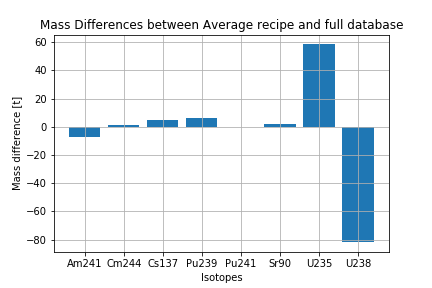
\includegraphics[width=0.45\textwidth]{./images/iso_mass.png}
    \caption{Mass difference between high resolution and simplified case for different isotopes.}
    \label{fig:iso_mass}
\end{figure}

\begin{figure}
    \centering
    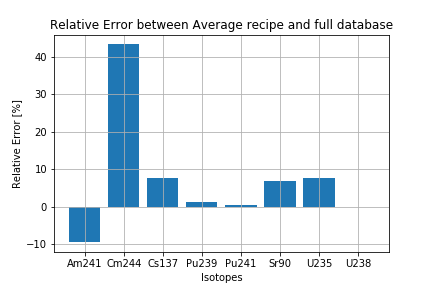
\includegraphics[width=0.45\textwidth]{./images/iso_rel.png}
    \caption{Relative error between high resolution and simplified case for different isotopes.}
    \label{fig:iso_rel}
\end{figure}

The same plots are generated for different plutonium
isotopes in Figures \ref{fig:pu_mass} and \ref{fig:pu_rel}.
The figures show that the simplified case under-calculates
all plutonium isotopes except for Pu-240, and that the
simplified case has 10 tons less plutonium than the
high-resolution case.

\begin{figure}
    \centering
    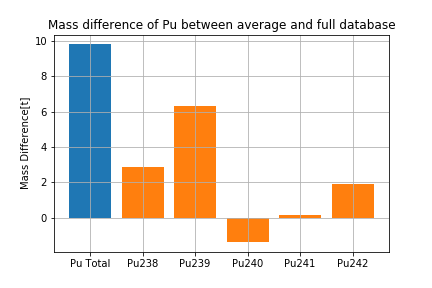
\includegraphics[width=0.45\textwidth]{./images/pu_mass.png}
    \caption{Mass difference between high resolution and simplified case for plutonium isotopes.}
    \label{fig:pu_mass}
\end{figure}

\begin{figure}
    \centering
    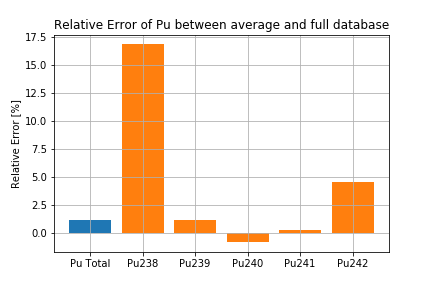
\includegraphics[width=0.45\textwidth]{./images/pu_rel.png}
    \caption{Relative error between high resolution and simplified case for plutonium isotopes.}
    \label{fig:pu_rel}
\end{figure}

\subsubsection{Waste Management Metrics}
The two major waste management metrics are radioactivity and
decay heat. Since the two metrics change in time, the metrics
are evaluated in three different times, in 2020, 2100 (short future),
and 3100 (far future). The results are shown in Table \ref{tab:wm} and
Figures \ref{fig:heat}, \ref{fig:act}, and \ref{fig:wm_err}.

\begin{table}[h]
    \centering
    \begin{tabular}{c|c|cc|c}
        \hline
        Metric & Year & HR case & Simpl. Case  & Rel. Err. [\%]\\
        \hline
        \multirow{3}{*}{\shortstack{Decay \\ Heat}} & 2020 & 61.31 & 53.90 & 12.08 \\
                                                    & 2100 & 24.27 & 23.63 & 2.63\\
                                                    & 3100 & 4.72 & 4.83 & -2.45\\
        \hline
        \multirow{3}{*}{\shortstack{Activity}} & 2020 & 6.76e20 & 6.33e20 & 6.27\\
                                               & 2100 & 9.28e19 & 8.76e19 & 5.59\\
                                               & 3100 & 5.54e18 & 5.654e18 & -2.02\\
        \hline
    \end{tabular}
    \caption{Decay heat and radioactivity values and errors for years 2020, 2100, and 3100.}
    \label{tab:wm}
\end{table}


Note that the error decreases with time, meaning that the error stems from the 
inaccuracy of the simplified case to take into account the short-lived fission
products (e.g. Cs-137, Sr-90), as shown in Figure \ref{fig:iso_rel}. The
error becomes negative after 2200, which is most likely due to the simplified
case having 10\% more Am-241 in its inventory.

\begin{figure}
    \centering
    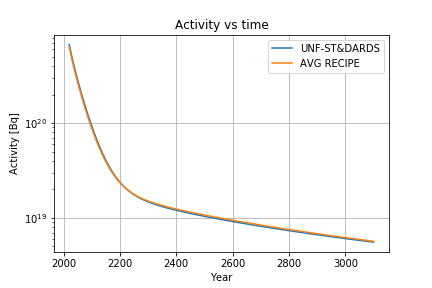
\includegraphics[width=0.45\textwidth]{./images/activity.png}
    \caption{Activity of the \gls{UNF} inventory for simplified and
            high resolution case.}
    \label{fig:act}
\end{figure}

\begin{figure}
    \centering
    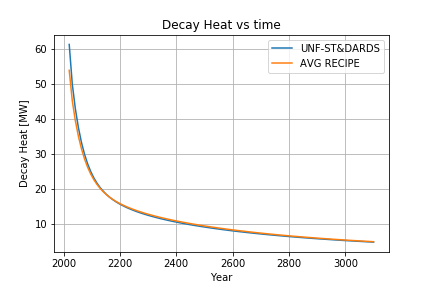
\includegraphics[width=0.45\textwidth]{./images/heat.png}
    \caption{Decay heat of the \gls{UNF} inventory for simplified
             and high resolution  case.}
    \label{fig:heat}
\end{figure}

\begin{figure}
    \centering
    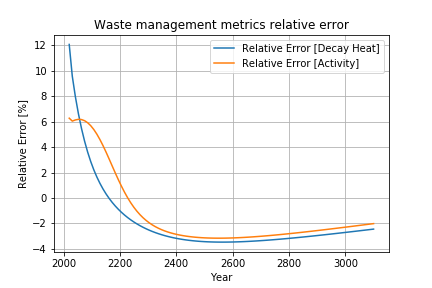
\includegraphics[width=0.45\textwidth]{./images/ha_err.png}
    \caption{Relative error of activity and decay heat of the
            \gls{UNF} inventory over time.}
    \label{fig:wm_err}
\end{figure}



\subsubsection{Fuel Cycle Analysis Metrics}
Given the isotopic compositions of the \gls{UNF} profile in 2020,
we calculate the equivalent Pu-239 for both cases, for
both spectra. The results are shown in Table \ref{tab:equiv}.
The figures show that the equivalent
Pu-239 difference between two cases is 7\% for thermal,
and less than 5\% for fast spectra.

\begin{table}[h]
    \centering
    \begin{tabular}{ccc}
        \hline
        Category & Equiv. Pu-239 ton & Rel. Error [\%] \\
        \hline
        HR thermal & 880.5 & \multirow{2}{*}{7.28}\\
        Simplified thermal & 816.4\\
        \hline
        HR fast & 1214.0 & \multirow{2}{*}{4.67}\\
        Simplified fast & 1157.3 &\\
        \hline
    \end{tabular}
    \caption{Equivalent Pu-239 ton value comparison for High-resolution and simplified case.}
    \label{tab:equiv}
\end{table}

To explain this error, we plotted every assembly and its
normalized equivalent Pu-239, shown in Figures \ref{fig:fast_all} and \ref{fig:thermal_all}.
The normalized equivalent Pu-239 is simply the 
total equivalent Pu-239 divided by the total mass
of the assembly.

\begin{figure}
    \centering
    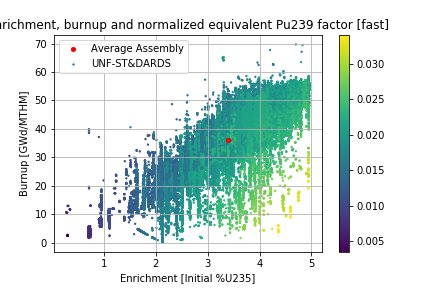
\includegraphics[width=0.45\textwidth]{./images/fast_all.png}
    \caption{All assemblies in the database and their normalized equivalent Pu-239 in a fast reactor.}
    \label{fig:fast_all}
\end{figure}

\begin{figure}
    \centering
    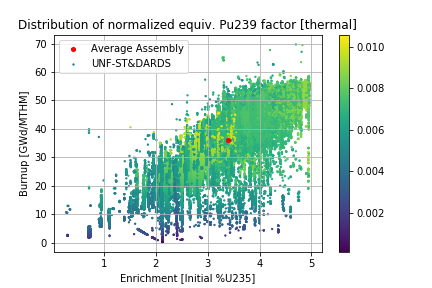
\includegraphics[width=0.45\textwidth]{./images/thermal_all.png}
    \caption{All assemblies in the database and their normalized equivalent Pu-239 in a thermal reactor.}
    \label{fig:thermal_all}
\end{figure}

The trend of the scatter plot shows that the \gls{UNF}
has a higher normalized equivalent Pu-239 when the
initial enrichment is high and the burnup low. One difference
to note is that in the fast spectrum the equivalent Pu-239
is higher than the thermal spectrum in higher burnup regions,
mostly due to the buildup of even plutonium isotopes with
higher burnup.

\section{Conclusion and Discussion}
In this paper, we compared the simplified \gls{UNF}
inventory and the high-resolution \gls{UNF} inventory
at 2020 by calculating the isotopic differences as well
as important metrics for waste management and fuel cycle analysis.
We conclude that the simplified inventory is not adequate for waste
management since the fission products and \glspl{MA}, that are sensitive to 
initial enrichment and burnup, are important when considering
waste management metrics, such as short and long-term decay heat and radioactivity.
Also, in waste management, it is important to consider each assembly separately,
thus having a total waste metric for the entire inventory is inadequate.
On the other hand, we found out that the simplified case can be a good
approximation of the \gls{UNF} inventory in terms of fuel cycle analysis,
given that the equivalent Pu-239 error for fast reactors are less than
5\%. Also, given that most fuel cycle simulators are fleet-based, and
because of the number of depletion calculations involved in a fuel cycle
simulation, it is hard for the reactor model to discharge a high-resolution \gls{UNF} profile.
The results from this paper support the view that depletion calculations
using recipes (pre-determined discharge compositions) are `good-enough' for preliminary fuel cycle simulations.

\section{Future Work}
We plan to couple \gls{UNF-STANDARDS} with Cyclus \cite{huff_fundamental_2016-1}, the agent-based fuel cycle simulator,
to perform fuel cycle transition scenarios using the simplified case
and the high-resolution case, to observe differences in transition
time and average reprocessing demand.

\section{Transition Scenario Analysis}
With the two different \gls{UNF} inventories with
the same mass but different composition, we perform
transition scenarios of the U.S. nuclear fleet from
a \gls{LWR} fleet to a \gls{SFR} fleet. We ran the
transition scenario starting in 2020 with the calculated
\gls{UNF} inventory and the current U.S. nuclear fleet.
To meet the increasing energy demand, more \glspl{LWR}
are deployed until the \glspl{SFR} become available.
We varied the nuclear energy demand growth rate and
\glspl{SFR} availability, as listed on table \ref{tab:param}.


\begin{table}[h]
    \centering
    \begin{tabular}{cc}
        \hline
        Parameters & Values \\
        \hline
        Energy Demand Growth Rate [\% per year] & 0, 0.5, 1, 1.5 \\
        \gls{SFR} available year & 2030, 2035, 2040, 2045, 2050\\
        Pre-2020 \gls{UNF} inventory & Precise \gls{UDB}, Recipe \gls{UDB}, None \\
        \hline
    \end{tabular}
    \caption{Parameters used for transition scenario}
    \label{tab:param}
\end{table}


\subsection{Results - Transition Scenario Analysis}
As expected, there was no observable difference between the
precise \gls{UDB} and the recipe \gls{UDB} case. As mentioned
above, the two cases differ very little in fissile content



\section{Acknowledgements}
The work done was funded through the Nuclear Engineering Science
Laboratory Synthesis (NESLS) program. We thank Kaushik Banerjee
from Oak Ridge National Laboratory for providing the data used
in this paper.

\bibliographystyle{ans}
\bibliography{bib}


\end{document}
